% !TEX encoding = UTF-8 Unicode
\documentclass[10pt,usepdftitle=false,aspectratio=169]{beamer}
\usepackage[left]{muibkitsec}
\usepackage{listings}

\usepackage{microtype}
\usepackage{graphbox}
\usepackage{booktabs} 

\usepackage{amsmath,amssymb,amsfonts,amsthm,mathtools}
\usepackage{algorithmic}
\usepackage{textcomp}
\usepackage{xcolor}
\usepackage{diagbox}
\usepackage{float, multirow}
\usepackage{tikz, pgfplots}
\usepackage{tikzsymbols}
\usetikzlibrary{spy}
\usepackage{subcaption}
\usepgfplotslibrary{groupplots}
\pgfplotsset{compat=newest}

% ------------------------------------------------------------------------
\title{Adversarial Label Flips}
%\subtitle{modified new beamer template}
\author{Matthias Dellago \& Maximilian Samsinger}
\date{22 January 2021}

% ------------------------------------------------------------------------

\begin{document}
\DeclarePairedDelimiter\abs{\lvert}{\rvert}%
\DeclarePairedDelimiter\norm{\lVert}{\rVert}%
\DeclarePairedDelimiter\ceil{\lceil}{\rceil}
\DeclarePairedDelimiter\floor{\lfloor}{\rfloor}

\begin{frame}[plain]
	\maketitle
\end{frame}	

%1x Introduction
%1x Slide Angriffe
%1x Slide Pytorch
%1x Slide Foolbox 
%1x Slide Datensätze
%1x Slide Pytorch
%
%
%1x Slide Architectures

%\begin{frame}[fragile]
%	\frametitle{Introduction/Reminder from last time}
%	\begin{columns}
%		\begin{column}{.5\columnwidth}
%			\begin{block}{Adversarial examples}
%				Generate adversarial examples. Create confusion matrix
%			\end{block}
%		\end{column}
%		\begin{column}{.5\columnwidth}
%			\begin{exampleblock}{Confusion matrix}
%				Confusion matrix from last presentation
%			\end{exampleblock}
%		\end{column}
%	\end{columns}
%\end{frame}

\begin{frame}[fragile]
	\frametitle{Standard sources on adversarial examples}
	\begin{columns}
		\begin{column}{.5\columnwidth}
			\begin{block}{Adversarial examples}
				Adversarial examples have been introduced in \cite{Szegedy13}.
			\end{block}
			\only<1-3>{\begin{alertblock}{Fast gradient sign method}
						FGSM has been introduced in \cite{goodfellow2014explaining}. \\
					\end{alertblock}}
			\only<4->{\begin{alertblock}{Projected gradient descent}
					Projected gradient descent is a popular, strong attack, which iteratively computes FGSM.
					It was introduces in \cite{madry2017towards}.
				\end{alertblock}}
		\end{column}
	\visible<2->{
		\begin{column}{.5\columnwidth}
			\begin{alertblock}{Fast gradient sign method}
				Modify an input image $x$  
				\[x + \epsilon\operatorname{sign}(\nabla_x\ J(\theta,x,y)). \] 
				using the loss function $J$.
			\end{alertblock}
		\end{column}}
	\end{columns}
	\only<1-3>{\source{[1] Intriguing properties of neural networks, 2014\\ {[2]} Explaining and harnessing adversarial examples, 2014}}
	\only<4->{\source{[1] Intriguing properties of neural networks, 2014\\ {[3]} Towards deep learning models resistant to adversarial attacks, 2018}}

\end{frame}

\begin{frame}[noframenumbering,fragile]
	\frametitle{Fast gradient sign method}
	\begin{tabular}{ccccc}
		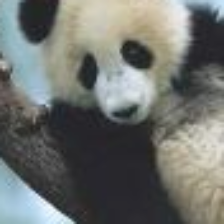
\includegraphics[align=c,width=0.28\columnwidth]{plots/panda_577.png} & \Huge{+} & \Huge{\textbf{$\epsilon$}}\ 
\includegraphics[align=c,width=0.28\columnwidth]{plots/nematode_082.png}\ & \Huge{=} & 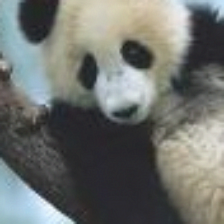
\includegraphics[align=c,width=0.28\columnwidth]{plots/gibbon_993.png} \\~\\
		\huge{Panda} &&\qquad \large{$\operatorname{sign}(\nabla_x\ J(\theta,x,y))$}&& \huge{Gibbon} \\
		(57.7\% confidence) &&&& (99.3\% confidence) 
	\end{tabular}
\end{frame}

\begin{frame}[fragile]
	\frametitle{What we want to do}
	Hier bitte die Matrix vom letzten Mal einfügen bitte!	
\end{frame}

\begin{frame}[fragile]
	\frametitle{Case study}
	
\end{frame}

\begin{frame}[fragile]
	\frametitle{What is Foolbox?}
	\begin{columns}
		\begin{column}{.45\columnwidth}
			\begin{block}{Foolbox}
				A suit of attacks is available with FoolBox! \cite{rauber2017foolbox}.
			\end{block}
		\end{column}
		\begin{column}{.55\columnwidth}
			\begin{alertblock}{Website}
				\url{https://foolbox.readthedocs.io}
			\end{alertblock}
		\end{column}
	\end{columns}
	\source{[4] Foolbox: A python toolbox to benchmark the robustness of machine learning models, 2017}
\end{frame}

\begin{frame}[fragile]
	\frametitle{Optional Slide 1: Data set}
	Some images for MNIST, Fashion-MNIST and CIFAR-10.
\end{frame}

\begin{frame}[fragile]
	\frametitle{Optional Slide 2: Convolutional neural networks}
	We use small convolutional neural networks \cite{lecun1999object} for the "easy" data sets. For CIFAR-10 we will use ResNet-18, a residual neural network \cite{he2016deep}, \cite{he2016identity}.
\end{frame}

\begin{frame}[allowframebreaks]
	\frametitle{References}
	\bibliographystyle{unsrt}
	\bibliography{literature}
\end{frame}


\end{document}
